\chapter{Review of Literature}
\label{chapter2}

\section{Grammatical Error Correction}
Grammatical error correction refers to the various tasks to correct the errors in the grammar \cite{ackah2016review}. 
Onwueguzie (2017) simply defined grammatical error correction task as the task to correct the sentence errors. The grammatical errors should be made to be different from other types of errors such as mispellings or mistakes in the omission of the characters in word structure (Onwueguzie, 2017). Grammatical errors are mainly the errors in grammar such as the structure or wrongly usage of subjective words or verbs (Onwueguzie, 2017). Leacock, Chodorow, Gamon and Tetreault (2014) characterize the normal grammatical errors as typographical errors or rule application errors and so on. Therefore, grammatical error correction is defined as the process of correcting any kinds of language usage errors in the grammar domain. 

Grammatical error correction is rather important for various reasons. According to \cite{nassaji2011correcting}, the importance of studying grammatical error correction mainly lies in the aspect that errors in grammar are rather common to see, which is a widespread issue to focus on. In addition, the grammatical errors in scholarly writing domain would generate huge negative influence on the academic writing performance including the message delivery and comprehension standards \cite{nassaji2011correcting}. 
\cite{truscott2007effect} argues that the grammatical error correction is rather effective and crucial to leverage the writers’ capability of writing accurately, which can also help to enhance writing confidence after suitable correction. 
\cite{truscott2007effect} further gets the research conclusion that grammatical error correction will also further enhance the learners’ capability in learning and capturing knowledge by properly arranging the message with better logic. 
It is found that the students being able to write more accurately tend to have better academic and learning performance \cite{fazio2001effect}.

\section{Natural Language Processing}

Natural language processing enjoys a long history and it is crucial to firstly identify its definitions. According to \cite{piotrowski2012natural}, natural language processing refers to the process of using computer systems to process and analyze the data about natural language. Tracing the history of the interactions between computers and language data coding, it can be found that the earliest natural language processing was in the 1950s when there was the article of “Computing Machinery and Intelligence” by Alan Turing (1950), making the formal starting point of the natural language processing. However, even before 1950, there were numerous scholars proposing the concepts of “language as a science” “the language relationship is the source of meaning creation” and “the shared norms to influence the decisions made by individuals” 
\cite{piotrowski2012natural}. These concepts paved the road that language could be structured and processed by turning the language systems into a digital system 
\cite{piotrowski2012natural}. Later since the 1980s, with the development of technology and evolution of society, natural language processing is then coming into use with the development of artificial intelligence \cite{kumar2011natural}. Artificial intelligence is the basic technology enabling the computers to comprehend and take advantage of the languages of human beings, which makes a possible for computers to have a dialogue with people \cite{bhirud2017grammar,kumar2011natural}. The great popularity of this technology was in 1990s while in the 21st century, the new NLP system was developed continuously, making the great progresses of the world \cite{kumar2011natural}.

\section{GEC Dataset}
Grammatical Error Correction has various datasets such as Conll and JFLEG \cite{ng2014conll,napoles2017jfleg}. The CoNLL-2013 dataset was defined to share the message of grammatical errors, so various task takers can share the correction works with evaluations of peers’ works. The primary goal of the CoNell dataset is to evaluate algorithms and systems in an automatic way enabling the function of correcting grammars for second-language English learners \cite{ng2014conll}. For JFLEG (full name of Fluency-Extended GUG Corpous), it is developed to evaluate the correction performance of various grammatical mistakes with 747 English sentences with 4 references separately \cite{napoles2017jfleg}. Two main goals for the grammatical performance checking based on this system are fluency and grammaticality \cite{napoles2017jfleg}. It is argued that the distinctiveness of JFLEG dataset is that it helps to present a comparable broader range of “language proficiency levels and uses holistic fluency edits” in the process of correcting the errors in grammar settings, which is also helpful to turn the original writing be more fluent and native \cite{napoles2017jfleg}. Therefore, from these two scholars’ opinions, it can be found that CoNll and JELEG dataset are both designed to test and correct the errors in grammar, but they share with each other the differences from aspects of core goals and functions.

\section{GEC Research}
There are also scholarly articles focusing on the work of grammatical error correction. \cite{bhirud2017grammar} argue that to better manage the process of grammatical error correction, it would be important to firstly characterize the common grammatical errors. There are 8 big categories of grammatical errors listed by \cite{bhirud2017grammar} named punctuational errors, constituents’ agreements errors, modifier being misplaced, pronominal reference being valuely presented, incorrect choice of words and no appropriate vocabulary, a shortage of the parallel structure, the sprawl issues in the sentences, and the problems lying in tense and modality agreements. However, \cite{soni2018systematic} categorize the grammar errors into several dimensions named frequency error, validity of text, standards of one error, the nature of one error, and error type overlapping problems. In the grammatical error checking process, it would be rather important to consider the role played by the grammatical error checker which constitutes both human quality checkers and artificial intelligence technology-based checkers \cite{bhirud2017grammar}. Grammar checking is the fundamental task to check where and what the problems are, and the severity of the errors \cite{bhirud2017grammar}. For a grammar quality checker, the normal working routines follow the following steps in the work: 
\begin{itemize}
    \item to segment and tokenize the sentences through cutting a whole sentence into several parts into the units of morphemes.
    \item to do the morphological analysis.
    \item to do the POS tagging job named part-of-speech tagging.
    \item and to parsing stage issues by checking the syntactic constraints in the overall hierarchical structure \cite{bhirud2017grammar}.
\end{itemize}

\cite{bhirud2017grammar} also develop three approaches for grammar checking named rule-based checker, data driven grammar checker and hybrid grammar checker. For rule-based checking mechanism, according to \cite{naber2003rule}, it needs the grammar checker to firstly characterize the features of grammar rules, develop the rules and then testing the rules, based on which it would compare the rules patterns within the existing sentence structure with the newly set language rules. It is argued that rule-based grammar checking began in the 1980s which focused on the area of language learning, and later, the rule-based grammar checking was applied in technological domain with the help of Microsoft Word to help to detect the grammar mistakes \cite{nazar2012google}. Rule-based grammar checking process has its advantages by overcoming the various barriers or obstacles through knowledge approaches or statistical approaches \cite{nazar2012google}. 

As for the data driven grammar checker, according to \cite{naber2003rule}, it refers to the process of checking grammar errors through drawing the data based on the journals, magazines and other online resources to get the corpus. \cite{naber2003rule} also points that the data-driven grammar checking approach has two sub methods named corpus based one and the one trying to check the input contents of texts through probabilistic methods. Data-driven grammar checking have two systems named MST and Malt system \cite{plank2010grammar}. For MST Parser, it is a graph-oriented dependency parser while the Malt system was a transition-based dependency parser, according to \cite{plank2010grammar}. The third one is hybrid method for grammar checking which refers to the process of utilizing the two approaches of data-driven approach and rule-based approach together at one time to check and correct the errors in one text \cite{bhirud2017grammar}. According to \cite{bhirud2017grammar}, the hybrid approach is more complex to use, asking for higher capabilities of quality checkers, but the overall grammar quality checking result can be better. 
Besides these three approaches of grammar error checking, it is argued by \cite{soni2018systematic} that with the development of technology, the grammar checking tools have also experienced the various stages from the writer’s workbench in the 1980s to the commercialized software package in the 1990s. In the 21st century with the fast development of web 2.0 and the associated information technology, there are a variety of the grammar checking techniques and tools such as Language Tool and other automatic grammar error detection systems on computers \cite{soni2018systematic}.

From these scholars’ ideas, it can be learned that the works of grammatical error checking have been experienced a huge development speed by capturing the trend of technology, web 2.0 and the application of specific approaches. Grammatical error checking is thus not only a process in theoretical domain but also the technical domain. However, the GEC approaches described above have their own drawbacks though they achieved state of the art at that time. The short comings are summarized below.
\begin{itemize}
    \item Rule-based approaches have poor generalization ability. It requires extensive effort to build the rule set. Regardless of the size of the rule set, considering the variability of the human languages, it seems impossible to cover all possible errors and there are lots of exception to the rules.
    \item Data driven approaches consume too much resources, e.g., memory. They also require large and domain adapted datasets to avoid the data-scarceness specific issues. In addition, they usually lack semantic information and favoring high-occurring events is not always the best way of detecting and correcting grammatical errors.
    \item Hybrid approaches maintain some drawbacks of rule-based approaches and data driven approaches since they ensemble both types. They may require many resources for statistical part as well as much time for rule design.
\end{itemize}
\section{Main Techniques}
The literature also identifies two main techniques for grammar error checking named Seq2seq Model and Long Short-term Memory Model \cite{lu2019advances}. 
We use Seq2seq model with LSTM based on the following reasons.
\begin{itemize}
    \item Seq2seq models with LSTM can generate arbitrary output sequences after seeing the entire input. They can even focus in on specific parts of the input automatically to help generate a useful translation.
    \item Seq2seq models have achieve great success in GEC area. Recent Seq2seq based GEC systems \cite{chollampatt2018multilayer,ge2018fluency,ge2018reaching}  can achieve human-level performance in GEC benchmarks.
\end{itemize}

\subsection{Seq2seq Model}
For Seq2seq model, according to \cite{lu2019advances}, it is used by selecting a foundational dataset which is given already, and then take the inputs situations into consideration to predict the outputs. The following Figure~\ref{fig:2} illustrates the example of the Seq2seq Model which incorporates both inputs situation and outputs situation \cite{lu2019advances}. The ABC are the input sequences while the WXY are the output sequences. Seq2seq model is also called encoder-decoder model and the purpose of the model is to translate some language texts from one to another based on some systematic processing systems \cite{schmaltz2016sentence}. It has the advantage of enabling the grammar checker to check the sentence-level errors and issues to a thorough way \cite{schmaltz2016sentence}. 
Other scholars \cite{szuba2001computational} state that Seq2Seq model is a rather useful framework for machine learning and machine translation which contains these steps named text summary, modeling of the conversations, capturing the images and so on. It is argued that Seq2Seq model is an encoder-decoder mechanism, so with the inputs to a system, it would also characterize the outputs \cite{szuba2001computational}. Therefore, it can be learned that the Seq2Seq model is a type of model enhancing the artificial intelligence technological performance \cite{szuba2001computational}. It also means that the model is helpful to characterize the comprehension of the natural languages in the process characterizing the grammar errors. 
\begin{figure}[ht]
    \centering
    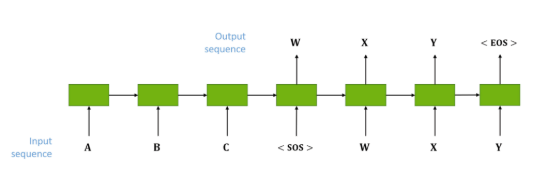
\includegraphics[width=\textwidth]{Seq2seqAE.png}
    \caption{Seq2Seq Architecture Example.}
    \label{fig:2}
\end{figure}

\subsection{Long Short-Term Memory}

The long short-term memory is an important neural network to better characterize the meanings in the area of deep learning \cite{hochreiter1997long}. Long short-term memory mechanism is widely applied in the studies of recognition of the handwriting. As shown in the following Figure 2, it can be found that the system is composed by inputs and outputs \cite{hochreiter1997long}. According to \cite{hochreiter1997long}, a comprehensive long short-term memory system is usually composed by various parts named cell, input gates, output gates and forget gate. The long short-term memory model has been applied in many situations including the memory training process and improving the learning effects. Applying the model in grammar error correction, the long short-term memory is thought to be rather crucial to leverage the overall quality standards when people are trying to memorize the grammar rules and seek further improvements \cite{zheng2016chinese}. Scholars of \cite{hochreiter1997long} point that long short-term memory is a kind of artificial recurrent neural network architecture, which is a key component to help to enhance deep learning. It is said by \cite{hochreiter1997long} that long short-term memory mechanism has its uniqueness by enhancing the feedback providing, so it can ensure the long-term entire sequence of data collection. It is thus an important perspective of grammar error collection. 


\begin{figure}[ht]
    \centering
    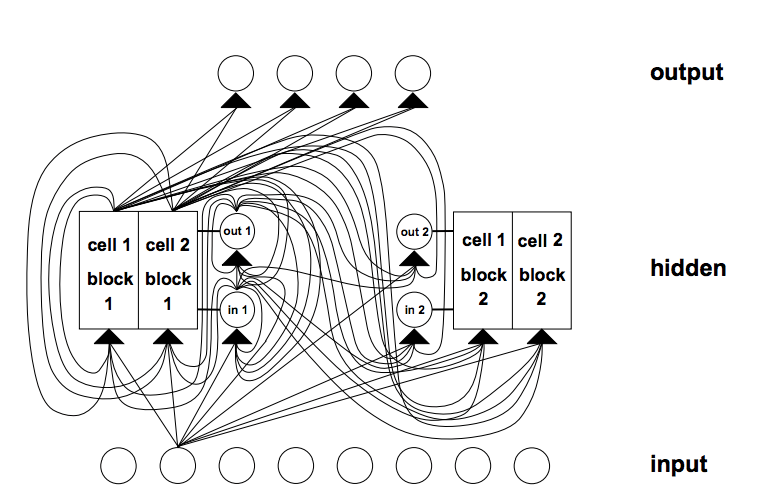
\includegraphics[width=\textwidth]{LSTM.png}
    \caption{Long Short-term Memory Model.}
    \label{fig:3}
\end{figure}